\documentclass[openany]{book}

\input{../../../latex_preambule_style/preambule}
\input{../../../latex_preambule_style/styleCoursCycle4}
\input{../../../latex_preambule_style/styleExercices}
\input{../../../latex_preambule_style/styleExercicesAideCompetences}
%\input{../../latex_preambule_style/styleCahier}
\input{../../../latex_preambule_style/bas_de_page_cycle4}
\input{../../../latex_preambule_style/algobox}


%%%%%%%%%%%%%%%  Affichage ou impression  %%%%%%%%%%%%%%%%%%
\newcommand{\impress}[2]{
\ifthenelse{\equal{#1}{1}}  %   1 imprime / affiche sur livre  -----    0 affiche sur cahier 
{%condition vraieé
#2
}% fin condition vraie
{%condition fausse
}% fin condition fausse
} % fin de la procédure
%%%%%%%%%%%%%%%  Affichage ou impression  %%%%%%%%%%%%%%%%%%

%%%%%%%%%%%%%%%%%%%%%%%%%%%%%%%%%%%%%%%%%%%%%%%%

\begin{document}


\begin{seance}[Trigonométrie]

\begin{description}
\item[$\square$] S’engager dans une démarche scientifique, observer, questionner, manipuler, expérimenter à l’aide de logiciels, émettre des hypothèses, une conjecture.
\end{description}
\end{seance}


\subsection{Connexion au support d'activité}


\begin{enumerate}
\item Se connecter à sacado.fr avec ses identifiants
\item Ouvrir le thème : Trigonométrie
\item Sélectionner l'activité : Découvrir le cosinus, le sinus, la tangente
\end{enumerate}


\subsection{Activité}

Le triangle $ADE$ est rectangle en $D$. On souhaite établir une relation entre l'angle $\widehat{DAE}$ et les cotés du triangle. 


\subsubsection{ Une figure dynamique}

\begin{enumerate}
\item Faire varier le point $E$. Vérifier que les longueurs des 3 cotés varient.
\item Faire varier, avec le curseur, l'angle $\alpha$. Vérifier que la longueur $AE$ ne varie pas.
\item Quel ensemble décrit le point $E$ ? \point{1}
\item Qu'est ce qu'une figure dynamique ? \point{1}
\end{enumerate}

\subsubsection{Une approche du cosinus}


\begin{enumerate}
\item Cocher la case du cosinus.
\item Faire varier le point $E$. Comment réagit la valeur du cosinus de $\widehat{DAE}$ ? \point{1}
\item Faire varier l'angle $\alpha$. Comment réagit la valeur du cosinus de $\widehat{DAE}$ ? \point{1}

\begin{Conjecture}
Le cosinus d'un angle est le quotient de la longueur du coté \ldots\ldots\ldots\ldots\ldots\ldots par la longueur de  \ldots\ldots\ldots\ldots\ldots\ldots\ldots\ldots
\end{Conjecture}


\item Quelle est la plus grande et la plus petite valeur du cosinus d'un angle aigu ? 
\end{enumerate}

\subsubsection{Une approche du sinus}


\begin{enumerate}
\item Décocher la case du cosinus et cocher la case du sinus.
\item Faire varier le point $E$. Comment réagit la valeur du sinus de $\widehat{DAE}$ ? \point{1}
\item Faire varier, avec le curseur, l'angle $\alpha$. Comment réagit la valeur du sinus de $\widehat{DAE}$ ? \point{1}
\begin{Conjecture}

Le sinus d'un angle est le quotient de la longueur du coté \ldots\ldots\ldots\ldots\ldots\ldots
par la longueur de  \ldots\ldots\ldots\ldots\ldots\ldots\ldots\ldots
\end{Conjecture}

\item Quelle est la plus grande et la plus petite valeur du sinus d'un angle aigu ? 
\end{enumerate}


\subsubsection{Une approche de la tangente}


\begin{enumerate}

\item Décocher la case du sinus et cocher la case de la tangente.
\item Faire varier le point $E$. Comment réagit la valeur de la tangente de $\widehat{DAE}$ ? \point{1}
\item Faire varier, avec le curseur, l'angle $\alpha$. Comment réagit la valeur de la tangente de $\widehat{DAE}$ ? \point{1}


\begin{Conjecture}
La tangente  d'un angle est le quotient de la longueur du coté \ldots\ldots\ldots\ldots\ldots\ldots par  la longueur du coté \ldots\ldots\ldots\ldots\ldots\ldots 
\end{Conjecture}


\item Quelle est la plus grande et la plus petite valeur de la tangente d'un angle aigu ? 
\end{enumerate}

\begin{Def}
Le  cosinus, le  sinus et la tangente  d'un angle sont des rapports de deux longueurs. 

\textbf{Réciproquement}, si on connait, un sinus ou un sinus ou une tangente, on peut alors connaitre un angle.
\end{Def}

\begin{Mt}
\begin{description}
\item[•] On utilise la touche \touche{Acos} ou \touche{Arccos} pour obtenir un angle à partir d'un cosinus.
\item[•] On utilise la touche \touche{Asin} ou \touche{Arcsin} pour obtenir un angle à partir d'un sinus.
\item[•] On utilise la touche \touche{Atan} ou \touche{Arctan} pour obtenir un angle à partir d'une tangente.
\end{description}
\end{Mt}

\begin{minipage}{0.48\linewidth}

\subsection{Démonstration}


\definecolor{yqyqyq}{rgb}{0.5019607843137255,0.5019607843137255,0.5019607843137255}
\definecolor{aqaqaq}{rgb}{0.6274509803921569,0.6274509803921569,0.6274509803921569}
\definecolor{qqwuqq}{rgb}{0.,0.39215686274509803,0.}
\definecolor{uuuuuu}{rgb}{0.26666666666666666,0.26666666666666666,0.26666666666666666}
\definecolor{ffqqqq}{rgb}{1.,0.,0.}
\begin{tikzpicture}[line cap=round,line join=round,>=triangle 45,x=1.0cm,y=1.0cm]
\clip(-2.280510827889474,-0.723406479627207) rectangle (6.199728096948752,6.946060248262661);
\draw [shift={(-1.8203428242160824,0.)},line width=2.pt,color=ffqqqq,fill=ffqqqq,fill opacity=0.8862745098039215] (0,0) -- (0.:0.6573828623905602) arc (0.:40.:0.6573828623905602) -- cycle;
\draw[line width=2.pt,color=qqwuqq,fill=qqwuqq,fill opacity=0.28999999165534973] (2.398914908076793,0.4648398798321881) -- (1.9340750282446049,0.46483987983218816) -- (1.9340750282446049,0.) -- (2.398914908076793,0.) -- cycle; 
\draw[line width=2.pt,color=qqwuqq,fill=qqwuqq,fill opacity=0.1899999976158142] (5.608083520797247,0.4648398798321881) -- (5.143243640965059,0.46483987983218816) -- (5.143243640965059,0.) -- (5.608083520797247,0.) -- cycle; 
\draw[line width=4.pt,color=ffqqqq,fill=ffqqqq,fill opacity=0.8899999856948853] (7.120064104295536,6.310590147951786) -- (11.064361278638897,6.310590147951786);
\draw (-3.1789340731565727,13.43223782384952) node[anchor=north west] {$AD=4.22\quad  \quad AE =5.51 \quad  \quad ED=3.54$};
\draw [line width=2.pt,color=aqaqaq] (-1.8203428242160824,0.)-- (2.398914908076793,0.);
\draw [line width=2.pt,color=aqaqaq] (-1.8203428242160824,0.)-- (2.398914908076793,3.540377607008838);
\draw [line width=2.pt,color=aqaqaq] (2.398914908076793,3.540377607008838)-- (2.398914908076793,0.);
\draw [line width=2.pt,color=aqaqaq] (-1.8203428242160824,0.)-- (5.608083520797247,0.);
\draw [line width=2.pt,color=yqyqyq] (-1.8203428242160824,0.)-- (5.608083520797246,6.233189806328275);
\draw [line width=2.pt,color=yqyqyq] (5.608083520797246,6.233189806328275)-- (5.608083520797247,0.);
\begin{scriptsize}
\draw [color=black] (-1.8203428242160824,0.)-- ++(-2.5pt,0 pt) -- ++(5.0pt,0 pt) ++(-2.5pt,-2.5pt) -- ++(0 pt,5.0pt);
\draw[color=black] (-1.973732158773879,0.4927518157953291) node {$A$};
\draw [color=black] (5.608083520797247,0.)-- ++(-2.5pt,0 pt) -- ++(5.0pt,0 pt) ++(-2.5pt,-2.5pt) -- ++(0 pt,5.0pt);
\draw[color=black] (5.695734569115989,-0.361845905312399) node {$B$};
\draw [fill=ffqqqq] (8.873085070670363,6.310590147951786) circle (2.5pt);
\draw [color=black] (2.398914908076793,3.540377607008838)-- ++(-2.5pt,0 pt) -- ++(5.0pt,0 pt) ++(-2.5pt,-2.5pt) -- ++(0 pt,5.0pt);
\draw[color=black] (1.9705650155694816,3.933055462305927) node {$E$};
\draw [color=uuuuuu] (2.398914908076793,0.)-- ++(-2.0pt,0 pt) -- ++(4.0pt,0 pt) ++(-2.0pt,-2.0pt) -- ++(0 pt,4.0pt);
\draw[color=uuuuuu] (2.364994733003818,-0.29610761907334304) node {$D$};
\draw [color=uuuuuu] (5.608083520797246,6.233189806328275)-- ++(-2.0pt,0 pt) -- ++(4.0pt,0 pt) ++(-2.0pt,-2.0pt) -- ++(0 pt,4.0pt);
\draw[color=uuuuuu] (5.761472855355045,6.584499673947853) node {$C$};
\end{scriptsize}
\end{tikzpicture}

\subsubsection{Le cosinus}

Démontrer, à l'aide du théorème de Thalès appliqué au triangle $ADE$ et $ABC$, que $$\frac{AD}{AE}=\frac{AB}{AC}$$

\begin{Th}
Dans tout triangle rectangle $ABC$, $$\cos \widehat{BAC} = \frac{ \text{ longueur du coté }\ldots\ldots\ldots\ldots\ldots\ldots}{ \text{ longueur de } \ldots\ldots\ldots\ldots\ldots\ldots\ldots}$$
\end{Th}

\end{minipage}
\hfill
\begin{minipage}{0.48\linewidth}
\subsubsection{Le sinus}

Démontrer, à l'aide du théorème de Thalès appliqué au triangle $ADE$ et $ABC$, que $$\frac{DE}{AE}=\frac{BC}{AC}$$

\begin{Th}
Dans tout triangle rectangle $ABC$, $$\sin \widehat{BAC} = \frac{ \text{ longueur du coté } \ldots\ldots\ldots\ldots\ldots\ldots}{ \text{ longueur de  } \ldots\ldots\ldots\ldots\ldots\ldots\ldots}$$
\end{Th}


\subsubsection{La tangente}

Démontrer, à l'aide du théorème de Thalès appliqué au triangle $ADE$ et $ABC$, que $$\frac{ED}{AD}=\frac{BC}{AB}$$

\begin{Th}
Dans tout triangle rectangle $ABC$, $$\tan \widehat{BAC} = \frac{ \text{ longueur du coté } \ldots\ldots\ldots\ldots\ldots\ldots}{ \text{ longueur du coté } \ldots\ldots\ldots\ldots\ldots\ldots\ldots}$$
\end{Th}
\end{minipage}

\begin{Rq}
Le  cosinus, le  sinus et la tangente permettent de calculer des longueurs et des angles dans un triangle rectangle.
\end{Rq}

\begin{seance}[Trigonométrie]

\begin{minipage}{0.60\linewidth}
\begin{description}
\item[$\square$] Reconnaitre les angles associés aux cotés d'un triangle rectangle
\item[$\square$] Extraire l'information d'une figure
\item[$\square$] Calculer le cosinus d'un angle
\item[$\square$] Calculer un angle à l'aide d'un cosinus
\end{description}
\end{minipage}
\hfill
\begin{minipage}{0.15\linewidth}

\includegraphics[scale=0.8]{qrcodeCote.png} 
\end{minipage}
\hfill
\begin{minipage}{0.15\linewidth}

\includegraphics[scale=0.8]{qrcodeCosinus.png} 
\end{minipage}

\end{seance}

\AD{1}{TR-169}

%\AD{1}{TR-84}
\EPC{1}{TR-219}{Chercher. Calculer.}


\EPC{1}{TR-209}{Représenter. Calculer.}

%\Exo{1}{TR-207}



\begin{seance}[Trigonométrie]

\begin{minipage}{0.68\linewidth}
\begin{description}
\item[$\square$] Reconnaitre les angles associés aux cotés d'un triangle rectangle
\item[$\square$] Extraire l'information d'une figure
\item[$\square$] Calculer le sinus d'un angle
\item[$\square$] Calculer un angle à l'aide d'un sinus
\end{description}

\end{minipage}
\hfill
\begin{minipage}{0.30\linewidth}

\includegraphics[scale=0.8]{qrcodeSinus.png} 
\end{minipage}
\end{seance}

\begin{minipage}{0.48\linewidth}
\Exo{1}{TR-212}
\end{minipage}
\hfill
\begin{minipage}{0.48\linewidth}
\Exo{1}{TR-220}
\end{minipage}

\Exo{1}{TR-215}


\begin{seance}[Trigonométrie]

\begin{minipage}{0.68\linewidth}
\begin{description}
\item[$\square$] Reconnaitre les angles associés aux cotés d'un triangle rectangle
\item[$\square$] Extraire l'information d'une figure
\item[$\square$] Calculer la tangente d'un angle
\item[$\square$] Calculer un angle à l'aide d'une tangente
\end{description}

\end{minipage}
\hfill
\begin{minipage}{0.30\linewidth}
\includegraphics[scale=0.8]{qrcodeTangente.png} 
\end{minipage}


\end{seance}

%\Exo{1}{TR-213}

\Exo{1}{TR-86}


\Exo{1}{TR-210}

\EPC{1}{TR-211}{Chercher. Calculer}


\begin{seance}[Trigonométrie]

\begin{description}
\item[Chercher] S'engager dans une démarche scientifique
\item[Modéliser] Comprendre et utiliser une simulation numérique ou géométrique.
\end{description}
\end{seance}

\Rec{1}{TR-216}

\begin{seance}[Trigonométrie]

\begin{description}
\item[Chercher] S'engager dans une démarche scientifique
\item[Chercher] Décomposer un problème en sous-problèmes
\item[Modéliser] Reconnaitre des situations de proportionnalités et résoudre les problèmes correspondants
\end{description}
\end{seance}

\DNB{1}{Pondichery}{TR-217}





\Rec{1}{TR-214}



\begin{seance}[Trigonométrie]

\begin{description}
\item[Représenter] Changer de registre 
\end{description}
\end{seance}

\Exo{1}{TR-208}

\DNB{1}{Asie}{TR-218}


\begin{seance}[Trigonométrie]

\begin{description}
\item[Chercher] S'engager dans une démarche scientifique
\item[Chercher] Décomposer un problème en sous-problèmes
\item[Modéliser] Reconnaitre des situations de proportionnalités et résoudre les problèmes correspondants
\end{description}
\end{seance}

Je souhaiterais fabriquer un de ces trois porte-manteaux que j'ai vu en photo sur Internet. 

J'ai contacté des artisans qui me demandent les plans et les vues de coupes et de face, chacun sur une feuille A4. 

Les dimensions doivent être à l'échelle.

J'aimerai bien aussi avoir une idée de prix, de l'encombrement au sol pour les porte-manteaux en pied, le débattement  pour le porte-manteau mural.


\begin{minipage}{0.33\linewidth}
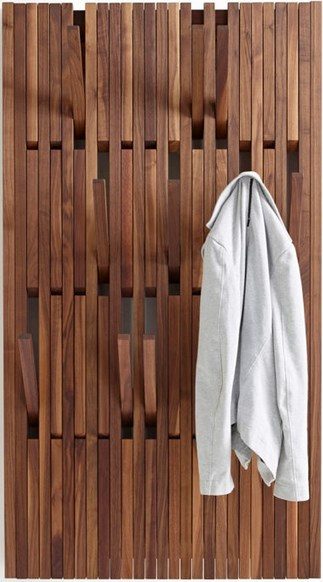
\includegraphics[scale=0.5]{blu-dot-coat-rack.jpg}  
\end{minipage}
\hfill
\begin{minipage}{0.33\linewidth}
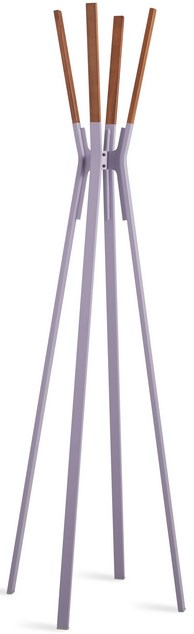
\includegraphics[scale=0.8]{porte-manteau.jpg}
\end{minipage}
\hfill
\begin{minipage}{0.33\linewidth}
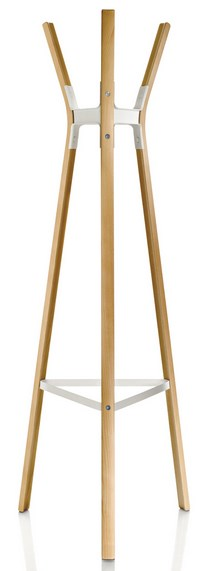
\includegraphics[scale=0.8]{porte-manteau-bois.jpg}
\end{minipage}

J'ai bien commencé une ébauche mais je n'ai pas trop le temps de tout faire ! Si ça vous tente.... on lance la production !

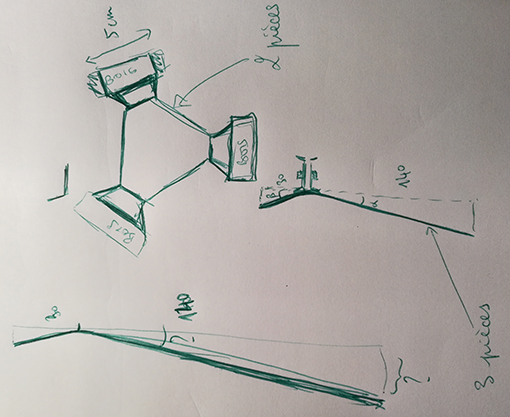
\includegraphics[scale=0.6]{ebauche.jpg} 



\begin{seance}[Trigonométrie]

\subsection{Synthèse}
\end{seance}

\begin{minipage}{0.70\linewidth}

\sectioncolor{eduscol4P}{{\normalsize Cosinus d'un angle}}

Dans le triangle \ldots \ldots \ldots rectangle en B , $\cos \widehat{BAC} = \ldots$

\sectioncolor{eduscol4P}{{\normalsize Sinus d'un angle}}

Dans le triangle \ldots \ldots \ldots rectangle en B , $\sin \widehat{BAC} = \ldots$

\sectioncolor{eduscol4P}{{\normalsize Tangente d'un angle}}

Dans le triangle \ldots \ldots \ldots rectangle en B , $\tan \widehat{BAC} = \ldots$
\end{minipage}
\hfill
\begin{minipage}{0.8\linewidth}
\definecolor{qqwuqq}{rgb}{0.,0.39215686274509803,0.}
\begin{tikzpicture}[line cap=round,line join=round,>=triangle 45,x=1.0cm,y=1.0cm]
\draw [shift={(2.,-1.)},line width=2.pt,fill=black,fill opacity=0.10000000149011612] (0,0) -- (0.:0.6) arc (0.:36.86989764584402:0.6) -- cycle;
\draw[line width=2.pt,color=qqwuqq,fill=qqwuqq,fill opacity=0.10000000149011612] (6.,-0.5757359312880715) -- (5.575735931288071,-0.5757359312880714) -- (5.575735931288071,-1.) -- (6.,-1.) -- cycle; 
\draw [line width=1.pt] (2.,-1.)-- (6.,-1.);
\draw [line width=1.pt] (6.,-1.)-- (6.,2.);
\draw [line width=1.pt] (6.,2.)-- (2.,-1.);
\begin{scriptsize}
\draw [color=black] (2.,-1.)-- ++(-2.5pt,0 pt) -- ++(5.0pt,0 pt) ++(-2.5pt,-2.5pt) -- ++(0 pt,5.0pt);
\draw[color=black] (1.7,-0.71) node {$A$};
\draw [color=black] (6.,-1.)-- ++(-2.5pt,0 pt) -- ++(5.0pt,0 pt) ++(-2.5pt,-2.5pt) -- ++(0 pt,5.0pt);
\draw[color=black] (6.14,-1.03) node {$B$};
\draw [color=black] (6.,2.)-- ++(-2.5pt,0 pt) -- ++(5.0pt,0 pt) ++(-2.5pt,-2.5pt) -- ++(0 pt,5.0pt);
\draw[color=black] (6.14,2.37) node {$C$};
\end{scriptsize}
\end{tikzpicture}
\end{minipage}


\sectioncolor{eduscol4B}{Calcul d'une longueur}

\vspace{0.3cm}

\begin{minipage}{0.68\linewidth}
\begin{enonce}[eduscol4B]

Le triangle $ABC$ est rectangle en $B$. \'A l'aide des informations, on souhaite calculer la valeur exacte de :

\begin{enumerate}
\item $AC$ et en donner une valeur approchée à $10^{-2}$ près.
\item $BC$ et en donner une valeur approchée à $10^{-2}$ près.
\end{enumerate}

\end{enonce}

\textbf{Solution.}
\begin{enumerate}
\item Le triangle $ABC$ est rectangle en $B$ donc $\cos \widehat{BAC} = \ldots \ldots$ 

donc $\cos 40\deg =  \ldots \ldots$ 

donc \fbox{$AC=  \ldots \ldots \ldots \ldots$}. 

Avec la calculatrice, $AC \approx  \ldots \ldots$.
\item Le triangle $ABC$ est rectangle en $B$ donc $\tan \widehat{BAC} =  \ldots \ldots$ 

donc $ \ldots \ldots = BC$ 

donc \fbox{$ \ldots \ldots = BC$}. 

Avec la calculatrice, $BC \approx  \ldots \ldots \ldots \ldots$.
\end{enumerate}


\end{minipage}
\hfill
\begin{minipage}{0.28\linewidth}
\definecolor{qqwuqq}{rgb}{0.,0.39215686274509803,0.}
\begin{tikzpicture}[line cap=round,line join=round,>=triangle 45,x=1.0cm,y=1.0cm]
\draw [shift={(2.,-1.)},line width=2.pt,fill=black,fill opacity=0.10000000149011612] (0,0) -- (0.:0.6) arc (0.:36.86989764584402:0.6) -- cycle;
\draw[line width=2.pt,color=qqwuqq,fill=qqwuqq,fill opacity=0.10000000149011612] (6.,-0.5757359312880715) -- (5.575735931288071,-0.5757359312880714) -- (5.575735931288071,-1.) -- (6.,-1.) -- cycle; 
\draw [line width=1.pt] (2.,-1.)-- (6.,-1.);
\draw [line width=1.pt] (6.,-1.)-- (6.,2.);
\draw [line width=1.pt] (6.,2.)-- (2.,-1.);
\draw (2.6,-0.46) node[anchor=north west] {$40\deg$};
\draw (3.76,-1) node[anchor=north west] {$5$};
\begin{scriptsize}
\draw [color=black] (2.,-1.)-- ++(-2.5pt,0 pt) -- ++(5.0pt,0 pt) ++(-2.5pt,-2.5pt) -- ++(0 pt,5.0pt);
\draw[color=black] (1.7,-0.71) node {$A$};
\draw [color=black] (6.,-1.)-- ++(-2.5pt,0 pt) -- ++(5.0pt,0 pt) ++(-2.5pt,-2.5pt) -- ++(0 pt,5.0pt);
\draw[color=black] (6.14,-0.63) node {$B$};
\draw [color=black] (6.,2.)-- ++(-2.5pt,0 pt) -- ++(5.0pt,0 pt) ++(-2.5pt,-2.5pt) -- ++(0 pt,5.0pt);
\draw[color=black] (6.14,2.37) node {$C$};
\end{scriptsize}
\end{tikzpicture}
\end{minipage}



\sectioncolor{eduscol4B}{Calcul d'une mesure d'angle}

\vspace{0.3cm}

\begin{minipage}{0.68\linewidth}

\begin{enonce}[eduscol4B]

Le triangle $ABC$ est rectangle en $B$. 

Calculer la valeur exacte de $\widehat{BAC}$, puis en donner une valeur approchée à $10^{-2}$.
\end{enonce}

\textbf{Solution.}

Le triangle $ABC$ est rectangle en $B$ donc $\sin \widehat{BAC} =  \ldots \ldots$ 

donc $\sin  \widehat{BAC} =  \ldots \ldots  \ldots \ldots=  \ldots \ldots$. 

A l'aide de la calculatrice, on tape  \ldots \ldots \ldots \ldots

donc  \fbox{$\widehat{BAC} \approx  \ldots \ldots \ldots \ldots \deg$}. 




\end{minipage}
\hfill
\begin{minipage}{0.28\linewidth}
\definecolor{qqwuqq}{rgb}{0.,0.39215686274509803,0.}
\begin{tikzpicture}[line cap=round,line join=round,>=triangle 45,x=1.0cm,y=1.0cm]
\draw [shift={(2.,-1.)},line width=2.pt,fill=black,fill opacity=0.10000000149011612] (0,0) -- (0.:0.5454545454545454) arc (0.:36.86989764584402:0.5454545454545454) -- cycle;
\draw[line width=2.pt,color=qqwuqq,fill=qqwuqq,fill opacity=0.10000000149011612] (6.,-0.614305392080065) -- (5.614305392080065,-0.614305392080065) -- (5.614305392080065,-1.) -- (6.,-1.) -- cycle; 
\draw [line width=1.pt] (2.,-1.)-- (6.,-1.);
\draw [line width=1.pt] (6.,-1.)-- (6.,2.);
\draw [line width=1.pt] (6.,2.)-- (2.,-1.);
\draw (6.138181818181818,0.92) node[anchor=north west] {$3$};
\draw (3.5472727272727274,1.02909090909091) node[anchor=north west] {$5$};
\draw (2.674545454545455,-0.43) node[anchor=north west] {$?$};
\begin{scriptsize}
\draw [color=black] (2.,-1.)-- ++(-2.5pt,0 pt) -- ++(5.0pt,0 pt) ++(-2.5pt,-2.5pt) -- ++(0 pt,5.0pt);
\draw[color=black] (1.7290909090909092,-0.7436363636363619) node {$A$};
\draw [color=black] (6.,-1.)-- ++(-2.5pt,0 pt) -- ++(5.0pt,0 pt) ++(-2.5pt,-2.5pt) -- ++(0 pt,5.0pt);
\draw[color=black] (6.129090909090909,-0.6709090909090891) node {$B$};
\draw [color=black] (6.,2.)-- ++(-2.5pt,0 pt) -- ++(5.0pt,0 pt) ++(-2.5pt,-2.5pt) -- ++(0 pt,5.0pt);
\draw[color=black] (6.129090909090909,2.3290909090909095) node {$C$};
\end{scriptsize}
\end{tikzpicture}
\end{minipage}


\end{document}